\documentclass[11pt]{article}

% Mode is controlled by the `acl-mode` YAML field:
%   review   — anonymous, line numbers (default for submission)
%   final    — camera-ready, authors shown
%   preprint — non-anonymous, page numbers
% acl.sty handles: geometry (a4, 2.5cm margins), twocolumn, natbib,
%   caption, hyperref, bibliographystyle{acl_natbib}.
% Do NOT load those packages again here.
\usepackage[review]{acl}

% Packages from the official ACL template (acl_latex.tex) — safe to load after acl.sty
\usepackage{times}
\usepackage{latexsym}
\usepackage[T1]{fontenc}
\usepackage[utf8]{inputenc}
\usepackage{textcomp}   % euro sign and other symbols
\usepackage{microtype}
\usepackage{inconsolata}

% Math
\usepackage{amsmath}
\usepackage{amssymb}

% Tables — all three needed for pandoc's longtable output
\usepackage{longtable}
\usepackage{booktabs}
\usepackage{array}     % pandoc uses >{\raggedright\arraybackslash}p{} column types
\usepackage{calc}      % pandoc uses \real{} expressions for column widths
\usepackage{multirow}  % multi-row table cells

% longtable is incompatible with twocolumn mode (enforced by acl.sty).
% Use etoolbox hooks to temporarily switch to onecolumn around each longtable.
% The table will appear full-width on its own page segment.
\usepackage{etoolbox}
\BeforeBeginEnvironment{longtable}{\onecolumn}
\AfterEndEnvironment{longtable}{\twocolumn}

% Fix table caption numbering for longtable
\def\fnum@table{\tablename~\thetable}

% Graphics
\usepackage{graphicx}
\makeatletter
% pandoc uses \maxwidth and \maxheight when including images
\def\maxwidth{\ifdim\Gin@nat@width>\linewidth\linewidth\else\Gin@nat@width\fi}
\def\maxheight{\ifdim\Gin@nat@height>\textheight\textheight\else\Gin@nat@height\fi}
% Default figure placement
\def\fps@figure{htbp}
\makeatother

% Code blocks and inline code
\IfFileExists{upquote.sty}{\usepackage{upquote}}{}  % straight quotes in verbatim
\usepackage{fancyvrb}
\newcommand{\passthrough}[1]{#1}  % pandoc inline code

% Suppress date (ACL papers do not display a date)
\date{}

% pandoc: scale images to fit column width, preserving aspect ratio
\makeatletter
\newsavebox\pandoc@box
\newcommand*\pandocbounded[1]{%
  \sbox\pandoc@box{#1}%
  \Gscale@div\@tempa{\linewidth}{\wd\pandoc@box}%
  \ifdim\@tempa\p@<\p@\scalebox{\@tempa}{\usebox\pandoc@box}\else#1\fi%
}
\makeatother

% pandoc: tight lists (no extra space between items)
\providecommand{\tightlist}{%
  \setlength{\itemsep}{0pt}\setlength{\parskip}{0pt}}

\title{writeup}

% In review mode, acl.sty replaces the author block with
% "Anonymous ACL submission" automatically.
\author{
  Zachary Houghton \\
      University of California, Davis \\
        \texttt{znhoughton@ucdavis.edu}
     \And
  Kenji Sagae \\
      University of California, Davis \\
       \And
  Emily Morgan \\
      University of California, Davis \\
      }

\begin{document}
\maketitle

\begin{abstract}
(Abstract goes here.)
\end{abstract}

\section{Experiment 1: UP
Independently}\label{experiment-1-up-independently}

\subsection{Items}\label{items}

The classifier was trained to distinguish the hidden-state
representation of the particle \emph{up} from representations of other
tokens in the same sentence. Positive training examples consisted of
1,000 occurrences of standalone \emph{up} (i.e., functioning as a verbal
particle, as in \emph{pick up}), drawn from sentences in the C4 corpus.
Negative examples were 1,000 tokens randomly selected from the same
sentences, restricted to tokens whose decoded string consists entirely
of alphabetic characters (no numbers, punctuation, or special
characters), and excluding \emph{up} itself and any token containing
\emph{up} as a substring. The validation set was constructed identically
from a non-overlapping set of sentences (targeting 1,000 positive, 1,000
negative; exact counts vary slightly by model depending on how many
sentences yield a valid token position under each tokenizer --- see
Table~\ref{tbl-exp1-splits}).

The classifiers targeting OLMo-3 7B and the BabyLM models were trained
on the \textbf{same underlying sentences}, but the frequency and
predictability statistics used in the analyses were derived from the
respective corpus for each model (the C4 corpus for the OLMo model and
the BabyLM corpus for the BabyLM models). In other words, the training
sentences were identical across models, but the tokenization and corpus
statistics varied.

Split sizes by model are shown in Table~\ref{tbl-exp1-splits}. The test
set comprised verb--\emph{up} phrasal verb types (e.g., \emph{pick up},
\emph{set up}) with at least 20 occurrences in the corpus; up to 20
sentences were sampled per type. Corpus frequency and forward
transitional probability (FTP; \(P(\text{up} \mid V)\)) were derived
from the corpus matched to each model's training distribution. Because
the BabyLM corpus is smaller than C4, fewer V+up types attain a valid
(non-zero) FTP estimate under BabyLM statistics; only types with a valid
FTP are included in the analyses. Item-level statistics for the test set
are shown in Table~\ref{tbl-exp1-items}.

\begin{longtable}[]{@{}
  >{\raggedright\arraybackslash}p{(\linewidth - 14\tabcolsep) * \real{0.1379}}
  >{\raggedleft\arraybackslash}p{(\linewidth - 14\tabcolsep) * \real{0.1149}}
  >{\raggedleft\arraybackslash}p{(\linewidth - 14\tabcolsep) * \real{0.1149}}
  >{\raggedleft\arraybackslash}p{(\linewidth - 14\tabcolsep) * \real{0.0920}}
  >{\raggedleft\arraybackslash}p{(\linewidth - 14\tabcolsep) * \real{0.0920}}
  >{\raggedleft\arraybackslash}p{(\linewidth - 14\tabcolsep) * \real{0.1724}}
  >{\raggedleft\arraybackslash}p{(\linewidth - 14\tabcolsep) * \real{0.1264}}
  >{\raggedleft\arraybackslash}p{(\linewidth - 14\tabcolsep) * \real{0.1494}}@{}}

\caption{\label{tbl-exp1-splits}Train, validation, and test split sizes
for Experiment 1 (UP independently). Positive (pos) = standalone
\emph{up}; negative (neg) = other alphabetic token from the same
sentence. Test types = unique V+up types with ≥20 corpus occurrences;
items w/ FTP = subset with a valid (non-zero) FTP in the model-matched
corpus.}

\tabularnewline

\toprule\noalign{}
\begin{minipage}[b]{\linewidth}\raggedright
Model
\end{minipage} & \begin{minipage}[b]{\linewidth}\raggedleft
Train pos
\end{minipage} & \begin{minipage}[b]{\linewidth}\raggedleft
Train neg
\end{minipage} & \begin{minipage}[b]{\linewidth}\raggedleft
Val pos
\end{minipage} & \begin{minipage}[b]{\linewidth}\raggedleft
Val neg
\end{minipage} & \begin{minipage}[b]{\linewidth}\raggedleft
Test sentences
\end{minipage} & \begin{minipage}[b]{\linewidth}\raggedleft
Test types
\end{minipage} & \begin{minipage}[b]{\linewidth}\raggedleft
Items w/ FTP
\end{minipage} \\
\midrule\noalign{}
\endhead
\bottomrule\noalign{}
\endlastfoot
OLMo-3 7B & 1,000 & 1,000 & 992 & 1,000 & 81,586 & 4,082 & 3,927 \\
BabyLM 125M & 1,000 & 1,000 & 999 & 1,000 & 81,543 & 4,082 & 1,039 \\
BabyLM 350M & 1,000 & 1,000 & 999 & 1,000 & 81,543 & 4,082 & 1,039 \\
BabyLM 1.3B & 1,000 & 1,000 & 916 & 1,000 & 80,425 & 4,081 & 1,039 \\

\end{longtable}

\begin{longtable}[]{@{}
  >{\raggedright\arraybackslash}p{(\linewidth - 14\tabcolsep) * \real{0.1154}}
  >{\raggedleft\arraybackslash}p{(\linewidth - 14\tabcolsep) * \real{0.0769}}
  >{\raggedleft\arraybackslash}p{(\linewidth - 14\tabcolsep) * \real{0.1154}}
  >{\raggedright\arraybackslash}p{(\linewidth - 14\tabcolsep) * \real{0.1250}}
  >{\raggedleft\arraybackslash}p{(\linewidth - 14\tabcolsep) * \real{0.1058}}
  >{\raggedright\arraybackslash}p{(\linewidth - 14\tabcolsep) * \real{0.1538}}
  >{\raggedleft\arraybackslash}p{(\linewidth - 14\tabcolsep) * \real{0.1442}}
  >{\raggedleft\arraybackslash}p{(\linewidth - 14\tabcolsep) * \real{0.1635}}@{}}

\caption{\label{tbl-exp1-items}Item-level statistics for unique V+up
types in the test set, restricted to types with a valid FTP in the
model-matched corpus. Frequency is the raw corpus count; FTP = P(up
\textbar{} V); logit(FTP) = log(FTP / (1 − FTP)). OLMo uses C4
statistics; BabyLM uses BabyLM-corpus statistics (opt-125m shown as
representative).}

\tabularnewline

\toprule\noalign{}
\begin{minipage}[b]{\linewidth}\raggedright
Model
\end{minipage} & \begin{minipage}[b]{\linewidth}\raggedleft
N items
\end{minipage} & \begin{minipage}[b]{\linewidth}\raggedleft
Median freq
\end{minipage} & \begin{minipage}[b]{\linewidth}\raggedright
Freq range
\end{minipage} & \begin{minipage}[b]{\linewidth}\raggedleft
Median FTP
\end{minipage} & \begin{minipage}[b]{\linewidth}\raggedright
FTP range
\end{minipage} & \begin{minipage}[b]{\linewidth}\raggedleft
Med logit(FTP)
\end{minipage} & \begin{minipage}[b]{\linewidth}\raggedleft
Sents/type (med)
\end{minipage} \\
\midrule\noalign{}
\endhead
\bottomrule\noalign{}
\endlastfoot
BabyLM 125M & 1039 & 920 & 20 -- 390,086 & 0.0325 & 0.00003 -- 0.880 &
-3.40 & 20 \\
OLMo-3 7B & 3927 & 92 & 20 -- 390,086 & 0.0046 & 0.00003 -- 0.980 &
-5.38 & 20 \\

\end{longtable}

\subsection{Joint model --- first layer}\label{joint-model-first-layer}

\begin{longtable}[]{@{}
  >{\raggedright\arraybackslash}p{(\linewidth - 12\tabcolsep) * \real{0.1667}}
  >{\raggedright\arraybackslash}p{(\linewidth - 12\tabcolsep) * \real{0.2917}}
  >{\raggedleft\arraybackslash}p{(\linewidth - 12\tabcolsep) * \real{0.1250}}
  >{\raggedleft\arraybackslash}p{(\linewidth - 12\tabcolsep) * \real{0.1389}}
  >{\raggedleft\arraybackslash}p{(\linewidth - 12\tabcolsep) * \real{0.0972}}
  >{\raggedleft\arraybackslash}p{(\linewidth - 12\tabcolsep) * \real{0.0972}}
  >{\raggedleft\arraybackslash}p{(\linewidth - 12\tabcolsep) * \real{0.0833}}@{}}

\caption{\label{tbl-exp1-joint-first}Joint frequency × FTP model at the
first layer for UP independently. Estimates are from Bayesian linear
mixed-effects models (brms); \% \textgreater{} 0 indicates the
percentage of posterior samples with a positive estimate.}

\tabularnewline

\toprule\noalign{}
\begin{minipage}[b]{\linewidth}\raggedright
Model
\end{minipage} & \begin{minipage}[b]{\linewidth}\raggedright
Parameter
\end{minipage} & \begin{minipage}[b]{\linewidth}\raggedleft
Estimate
\end{minipage} & \begin{minipage}[b]{\linewidth}\raggedleft
Est.Error
\end{minipage} & \begin{minipage}[b]{\linewidth}\raggedleft
Q2.5
\end{minipage} & \begin{minipage}[b]{\linewidth}\raggedleft
Q97.5
\end{minipage} & \begin{minipage}[b]{\linewidth}\raggedleft
\% \textgreater{} 0
\end{minipage} \\
\midrule\noalign{}
\endhead
\bottomrule\noalign{}
\endlastfoot
OLMo-3 7B & Intercept & 18.582 & 0.011 & 18.561 & 18.603 & 100.0 \\
OLMo-3 7B & c\_log\_freq & -0.142 & 0.012 & -0.165 & -0.118 & 0.0 \\
OLMo-3 7B & c\_log\_ftp & -0.109 & 0.011 & -0.130 & -0.089 & 0.0 \\
OLMo-3 7B & c\_log\_freq:c\_log\_ftp & -0.087 & 0.011 & -0.108 & -0.066
& 0.0 \\
BabyLM 125M & Intercept & 10.769 & 0.011 & 10.747 & 10.791 & 100.0 \\
BabyLM 125M & c\_log\_freq & 0.028 & 0.011 & 0.006 & 0.050 & 99.3 \\
BabyLM 125M & c\_log\_ftp & -0.051 & 0.011 & -0.073 & -0.029 & 0.0 \\
BabyLM 125M & c\_log\_freq:c\_log\_ftp & -0.018 & 0.012 & -0.041 & 0.006
& 7.0 \\
BabyLM 350M & Intercept & 13.415 & 0.007 & 13.402 & 13.428 & 100.0 \\
BabyLM 350M & c\_log\_freq & -0.043 & 0.007 & -0.056 & -0.031 & 0.0 \\
BabyLM 350M & c\_log\_ftp & 0.037 & 0.007 & 0.024 & 0.050 & 100.0 \\
BabyLM 350M & c\_log\_freq:c\_log\_ftp & -0.006 & 0.007 & -0.020 & 0.007
& 18.3 \\
BabyLM 1.3B & Intercept & 16.385 & 0.026 & 16.334 & 16.437 & 100.0 \\
BabyLM 1.3B & c\_log\_freq & 0.176 & 0.026 & 0.126 & 0.229 & 100.0 \\
BabyLM 1.3B & c\_log\_ftp & -0.099 & 0.026 & -0.151 & -0.048 & 0.0 \\
BabyLM 1.3B & c\_log\_freq:c\_log\_ftp & 0.045 & 0.028 & -0.010 & 0.100
& 94.5 \\

\end{longtable}

\subsection{Joint model --- final layer}\label{joint-model-final-layer}

\begin{longtable}[]{@{}
  >{\raggedright\arraybackslash}p{(\linewidth - 12\tabcolsep) * \real{0.1667}}
  >{\raggedright\arraybackslash}p{(\linewidth - 12\tabcolsep) * \real{0.2917}}
  >{\raggedleft\arraybackslash}p{(\linewidth - 12\tabcolsep) * \real{0.1250}}
  >{\raggedleft\arraybackslash}p{(\linewidth - 12\tabcolsep) * \real{0.1389}}
  >{\raggedleft\arraybackslash}p{(\linewidth - 12\tabcolsep) * \real{0.0972}}
  >{\raggedleft\arraybackslash}p{(\linewidth - 12\tabcolsep) * \real{0.0972}}
  >{\raggedleft\arraybackslash}p{(\linewidth - 12\tabcolsep) * \real{0.0833}}@{}}

\caption{\label{tbl-exp1-joint-final}Joint frequency × FTP model at the
final layer for UP independently. Estimates are from Bayesian linear
mixed-effects models (brms); \% \textgreater{} 0 indicates the
percentage of posterior samples with a positive estimate.}

\tabularnewline

\toprule\noalign{}
\begin{minipage}[b]{\linewidth}\raggedright
Model
\end{minipage} & \begin{minipage}[b]{\linewidth}\raggedright
Parameter
\end{minipage} & \begin{minipage}[b]{\linewidth}\raggedleft
Estimate
\end{minipage} & \begin{minipage}[b]{\linewidth}\raggedleft
Est.Error
\end{minipage} & \begin{minipage}[b]{\linewidth}\raggedleft
Q2.5
\end{minipage} & \begin{minipage}[b]{\linewidth}\raggedleft
Q97.5
\end{minipage} & \begin{minipage}[b]{\linewidth}\raggedleft
\% \textgreater{} 0
\end{minipage} \\
\midrule\noalign{}
\endhead
\bottomrule\noalign{}
\endlastfoot
OLMo-3 7B & Intercept & 10.265 & 0.042 & 10.181 & 10.348 & 100.0 \\
OLMo-3 7B & c\_log\_freq & -0.541 & 0.047 & -0.633 & -0.446 & 0.0 \\
OLMo-3 7B & c\_log\_ftp & -1.562 & 0.042 & -1.645 & -1.478 & 0.0 \\
OLMo-3 7B & c\_log\_freq:c\_log\_ftp & 0.001 & 0.042 & -0.083 & 0.081 &
50.7 \\
BabyLM 125M & Intercept & 8.468 & 0.038 & 8.392 & 8.542 & 100.0 \\
BabyLM 125M & c\_log\_freq & -0.346 & 0.040 & -0.424 & -0.268 & 0.0 \\
BabyLM 125M & c\_log\_ftp & -0.222 & 0.040 & -0.300 & -0.146 & 0.0 \\
BabyLM 125M & c\_log\_freq:c\_log\_ftp & -0.050 & 0.041 & -0.129 & 0.030
& 11.3 \\
BabyLM 350M & Intercept & 8.798 & 0.036 & 8.728 & 8.871 & 100.0 \\
BabyLM 350M & c\_log\_freq & -0.432 & 0.038 & -0.504 & -0.357 & 0.0 \\
BabyLM 350M & c\_log\_ftp & 0.063 & 0.038 & -0.011 & 0.137 & 95.2 \\
BabyLM 350M & c\_log\_freq:c\_log\_ftp & -0.078 & 0.039 & -0.152 &
-0.002 & 2.2 \\
BabyLM 1.3B & Intercept & 8.383 & 0.043 & 8.298 & 8.465 & 100.0 \\
BabyLM 1.3B & c\_log\_freq & -0.219 & 0.044 & -0.305 & -0.132 & 0.0 \\
BabyLM 1.3B & c\_log\_ftp & -0.109 & 0.044 & -0.195 & -0.021 & 0.7 \\
BabyLM 1.3B & c\_log\_freq:c\_log\_ftp & -0.074 & 0.047 & -0.167 & 0.017
& 5.5 \\

\end{longtable}

\subsection{Joint model --- predicted surfaces
(linear)}\label{joint-model-predicted-surfaces-linear}

\begin{figure}

\centering{

\pandocbounded{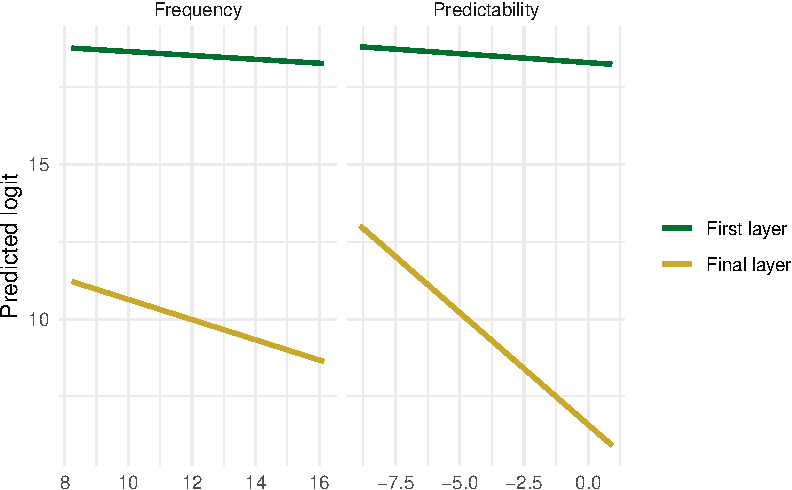
\includegraphics[keepaspectratio]{writeup_files/figure-pdf/fig-exp1-joint-surfaces-1.pdf}}

}

\caption{\label{fig-exp1-joint-surfaces}Predicted classifier logit as a
joint function of log-frequency and logit(FTP) from the linear joint
brms model (logit \textasciitilde{} c\_log\_freq × c\_log\_ftp), at the
first and final layers, for OLMo-3 7B (UP independently). Colour
indicates predicted logit; axes are back-transformed to the original
log/logit scale.}

\end{figure}%

\begin{figure}

\centering{

\pandocbounded{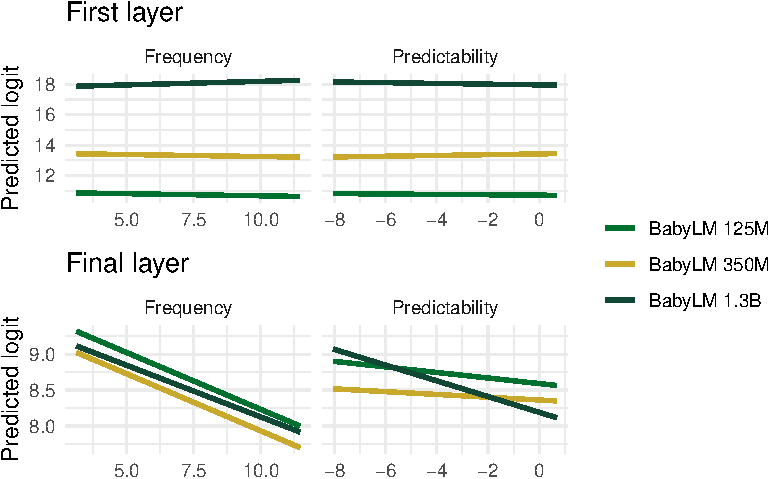
\includegraphics[keepaspectratio]{writeup_files/figure-pdf/fig-exp1-joint-surfaces-blm-1.pdf}}

}

\caption{\label{fig-exp1-joint-surfaces-blm}Predicted logit surfaces
from the linear joint brms model at the first and final layers for
BabyLM models (UP independently).}

\end{figure}%

\subsection{Polynomial joint model --- first
layer}\label{polynomial-joint-model-first-layer}

\begin{longtable}[]{@{}
  >{\raggedright\arraybackslash}p{(\linewidth - 12\tabcolsep) * \real{0.1667}}
  >{\raggedright\arraybackslash}p{(\linewidth - 12\tabcolsep) * \real{0.2917}}
  >{\raggedleft\arraybackslash}p{(\linewidth - 12\tabcolsep) * \real{0.1250}}
  >{\raggedleft\arraybackslash}p{(\linewidth - 12\tabcolsep) * \real{0.1389}}
  >{\raggedleft\arraybackslash}p{(\linewidth - 12\tabcolsep) * \real{0.0972}}
  >{\raggedleft\arraybackslash}p{(\linewidth - 12\tabcolsep) * \real{0.0972}}
  >{\raggedleft\arraybackslash}p{(\linewidth - 12\tabcolsep) * \real{0.0833}}@{}}

\caption{\label{tbl-exp1-poly-joint-first}Polynomial joint model (logit
\textasciitilde{} freq + freq² + FTP + FTP² + freq:FTP) at the first
layer for UP independently. All predictors are centered and scaled. \%
\textgreater{} 0 = percentage of posterior samples with a positive
estimate.}

\tabularnewline

\toprule\noalign{}
\begin{minipage}[b]{\linewidth}\raggedright
Model
\end{minipage} & \begin{minipage}[b]{\linewidth}\raggedright
Parameter
\end{minipage} & \begin{minipage}[b]{\linewidth}\raggedleft
Estimate
\end{minipage} & \begin{minipage}[b]{\linewidth}\raggedleft
Est.Error
\end{minipage} & \begin{minipage}[b]{\linewidth}\raggedleft
Q2.5
\end{minipage} & \begin{minipage}[b]{\linewidth}\raggedleft
Q97.5
\end{minipage} & \begin{minipage}[b]{\linewidth}\raggedleft
\% \textgreater{} 0
\end{minipage} \\
\midrule\noalign{}
\endhead
\bottomrule\noalign{}
\endlastfoot
OLMo-3 7B & Intercept & 18.532 & 0.014 & 18.505 & 18.560 & 100.0 \\
OLMo-3 7B & c\_log\_freq & -0.053 & 0.014 & -0.079 & -0.027 & 0.0 \\
OLMo-3 7B & Ic\_log\_freqE2 & -0.043 & 0.009 & -0.061 & -0.026 & 0.0 \\
OLMo-3 7B & c\_log\_ftp & -0.184 & 0.012 & -0.206 & -0.161 & 0.0 \\
OLMo-3 7B & Ic\_log\_ftpE2 & 0.111 & 0.008 & 0.094 & 0.127 & 100.0 \\
OLMo-3 7B & c\_log\_freq:c\_log\_ftp & -0.130 & 0.014 & -0.157 & -0.102
& 0.0 \\
BabyLM 125M & Intercept & 10.754 & 0.016 & 10.722 & 10.786 & 100.0 \\
BabyLM 125M & c\_log\_freq & 0.028 & 0.011 & 0.006 & 0.050 & 99.3 \\
BabyLM 125M & Ic\_log\_freqE2 & 0.010 & 0.009 & -0.008 & 0.028 & 85.6 \\
BabyLM 125M & c\_log\_ftp & -0.050 & 0.011 & -0.074 & -0.029 & 0.0 \\
BabyLM 125M & Ic\_log\_ftpE2 & 0.006 & 0.008 & -0.009 & 0.021 & 78.1 \\
BabyLM 125M & c\_log\_freq:c\_log\_ftp & -0.023 & 0.013 & -0.048 & 0.002
& 3.5 \\
BabyLM 350M & Intercept & 13.436 & 0.010 & 13.417 & 13.455 & 100.0 \\
BabyLM 350M & c\_log\_freq & -0.044 & 0.007 & -0.057 & -0.031 & 0.0 \\
BabyLM 350M & Ic\_log\_freqE2 & -0.010 & 0.005 & -0.021 & 0.000 & 2.8 \\
BabyLM 350M & c\_log\_ftp & 0.036 & 0.007 & 0.023 & 0.049 & 100.0 \\
BabyLM 350M & Ic\_log\_ftpE2 & -0.012 & 0.004 & -0.020 & -0.003 & 0.4 \\
BabyLM 350M & c\_log\_freq:c\_log\_ftp & 0.002 & 0.007 & -0.013 & 0.016
& 58.7 \\
BabyLM 1.3B & Intercept & 16.363 & 0.038 & 16.290 & 16.437 & 100.0 \\
BabyLM 1.3B & c\_log\_freq & 0.177 & 0.027 & 0.125 & 0.229 & 100.0 \\
BabyLM 1.3B & Ic\_log\_freqE2 & 0.009 & 0.021 & -0.033 & 0.050 & 65.8 \\
BabyLM 1.3B & c\_log\_ftp & -0.098 & 0.027 & -0.150 & -0.045 & 0.0 \\
BabyLM 1.3B & Ic\_log\_ftpE2 & 0.014 & 0.017 & -0.020 & 0.048 & 78.9 \\
BabyLM 1.3B & c\_log\_freq:c\_log\_ftp & 0.037 & 0.029 & -0.022 & 0.094
& 89.3 \\

\end{longtable}

\subsection{Polynomial joint model --- final
layer}\label{polynomial-joint-model-final-layer}

\begin{longtable}[]{@{}
  >{\raggedright\arraybackslash}p{(\linewidth - 12\tabcolsep) * \real{0.1667}}
  >{\raggedright\arraybackslash}p{(\linewidth - 12\tabcolsep) * \real{0.2917}}
  >{\raggedleft\arraybackslash}p{(\linewidth - 12\tabcolsep) * \real{0.1250}}
  >{\raggedleft\arraybackslash}p{(\linewidth - 12\tabcolsep) * \real{0.1389}}
  >{\raggedleft\arraybackslash}p{(\linewidth - 12\tabcolsep) * \real{0.0972}}
  >{\raggedleft\arraybackslash}p{(\linewidth - 12\tabcolsep) * \real{0.0972}}
  >{\raggedleft\arraybackslash}p{(\linewidth - 12\tabcolsep) * \real{0.0833}}@{}}

\caption{\label{tbl-exp1-poly-joint-final}Polynomial joint model (logit
\textasciitilde{} freq + freq² + FTP + FTP² + freq:FTP) at the final
layer for UP independently. All predictors are centered and scaled. \%
\textgreater{} 0 = percentage of posterior samples with a positive
estimate.}

\tabularnewline

\toprule\noalign{}
\begin{minipage}[b]{\linewidth}\raggedright
Model
\end{minipage} & \begin{minipage}[b]{\linewidth}\raggedright
Parameter
\end{minipage} & \begin{minipage}[b]{\linewidth}\raggedleft
Estimate
\end{minipage} & \begin{minipage}[b]{\linewidth}\raggedleft
Est.Error
\end{minipage} & \begin{minipage}[b]{\linewidth}\raggedleft
Q2.5
\end{minipage} & \begin{minipage}[b]{\linewidth}\raggedleft
Q97.5
\end{minipage} & \begin{minipage}[b]{\linewidth}\raggedleft
\% \textgreater{} 0
\end{minipage} \\
\midrule\noalign{}
\endhead
\bottomrule\noalign{}
\endlastfoot
OLMo-3 7B & Intercept & 10.139 & 0.056 & 10.028 & 10.248 & 100.0 \\
OLMo-3 7B & c\_log\_freq & -0.577 & 0.057 & -0.687 & -0.464 & 0.0 \\
OLMo-3 7B & Ic\_log\_freqE2 & 0.091 & 0.035 & 0.021 & 0.160 & 99.5 \\
OLMo-3 7B & c\_log\_ftp & -1.617 & 0.049 & -1.713 & -1.523 & 0.0 \\
OLMo-3 7B & Ic\_log\_ftpE2 & 0.087 & 0.034 & 0.022 & 0.153 & 99.6 \\
OLMo-3 7B & c\_log\_freq:c\_log\_ftp & -0.119 & 0.055 & -0.226 & -0.012
& 1.5 \\
BabyLM 125M & Intercept & 8.425 & 0.055 & 8.319 & 8.535 & 100.0 \\
BabyLM 125M & c\_log\_freq & -0.316 & 0.039 & -0.394 & -0.239 & 0.0 \\
BabyLM 125M & Ic\_log\_freqE2 & -0.089 & 0.031 & -0.149 & -0.030 &
0.2 \\
BabyLM 125M & c\_log\_ftp & -0.189 & 0.038 & -0.265 & -0.115 & 0.0 \\
BabyLM 125M & Ic\_log\_ftpE2 & 0.138 & 0.025 & 0.088 & 0.188 & 100.0 \\
BabyLM 125M & c\_log\_freq:c\_log\_ftp & -0.087 & 0.044 & -0.172 &
-0.001 & 2.4 \\
BabyLM 350M & Intercept & 8.771 & 0.054 & 8.669 & 8.877 & 100.0 \\
BabyLM 350M & c\_log\_freq & -0.400 & 0.037 & -0.473 & -0.329 & 0.0 \\
BabyLM 350M & Ic\_log\_freqE2 & -0.101 & 0.029 & -0.160 & -0.044 &
0.0 \\
BabyLM 350M & c\_log\_ftp & 0.096 & 0.038 & 0.021 & 0.171 & 99.3 \\
BabyLM 350M & Ic\_log\_ftpE2 & 0.131 & 0.024 & 0.081 & 0.178 & 100.0 \\
BabyLM 350M & c\_log\_freq:c\_log\_ftp & -0.111 & 0.040 & -0.191 &
-0.032 & 0.4 \\
BabyLM 1.3B & Intercept & 8.329 & 0.063 & 8.204 & 8.450 & 100.0 \\
BabyLM 1.3B & c\_log\_freq & -0.180 & 0.043 & -0.266 & -0.094 & 0.0 \\
BabyLM 1.3B & Ic\_log\_freqE2 & -0.124 & 0.034 & -0.191 & -0.056 &
0.0 \\
BabyLM 1.3B & c\_log\_ftp & -0.062 & 0.044 & -0.148 & 0.025 & 8.0 \\
BabyLM 1.3B & Ic\_log\_ftpE2 & 0.186 & 0.029 & 0.131 & 0.243 & 100.0 \\
BabyLM 1.3B & c\_log\_freq:c\_log\_ftp & -0.126 & 0.048 & -0.220 &
-0.033 & 0.3 \\

\end{longtable}

\subsection{Polynomial joint model --- predicted
surfaces}\label{polynomial-joint-model-predicted-surfaces}

\begin{figure}

\centering{

\pandocbounded{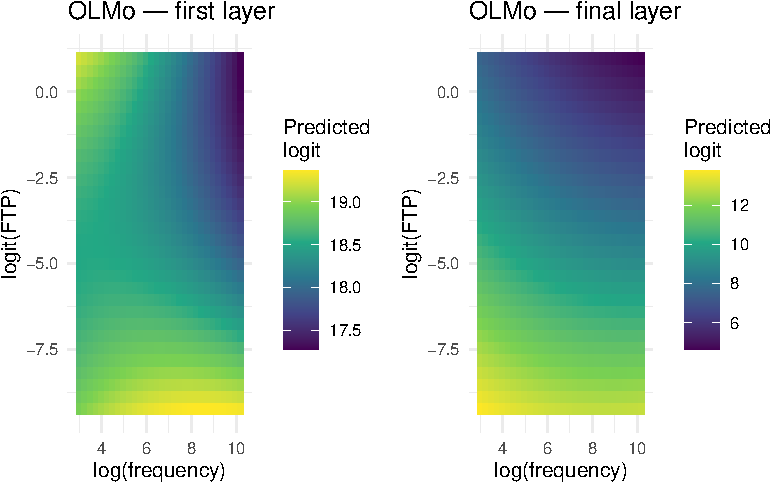
\includegraphics[keepaspectratio]{writeup_files/figure-pdf/fig-exp1-poly-joint-surfaces-1.pdf}}

}

\caption{\label{fig-exp1-poly-joint-surfaces}Predicted logit surfaces
from the polynomial joint brms model at the first and final layers for
OLMo-3 7B (UP independently).}

\end{figure}%

\begin{figure}

\centering{

\pandocbounded{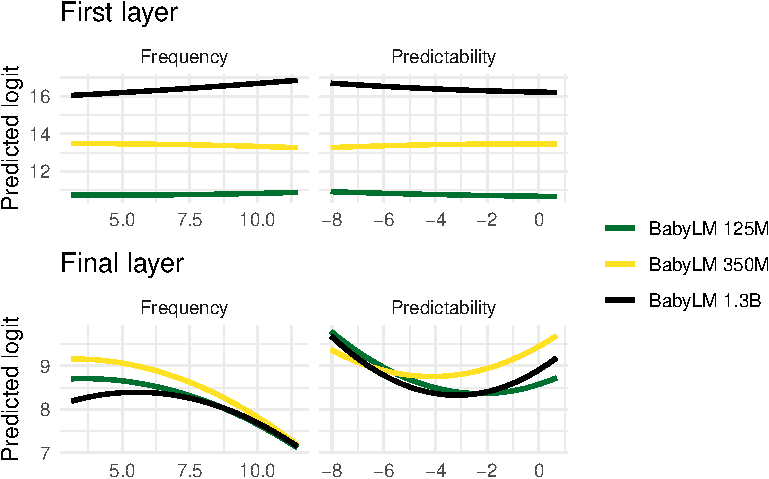
\includegraphics[keepaspectratio]{writeup_files/figure-pdf/fig-exp1-poly-joint-surfaces-blm-1.pdf}}

}

\caption{\label{fig-exp1-poly-joint-surfaces-blm}Predicted logit
surfaces from the polynomial joint brms model at the first and final
layers for BabyLM models (UP independently).}

\end{figure}%

\subsection{Frequency effect across
layers}\label{frequency-effect-across-layers}

\begin{figure}

\centering{

\pandocbounded{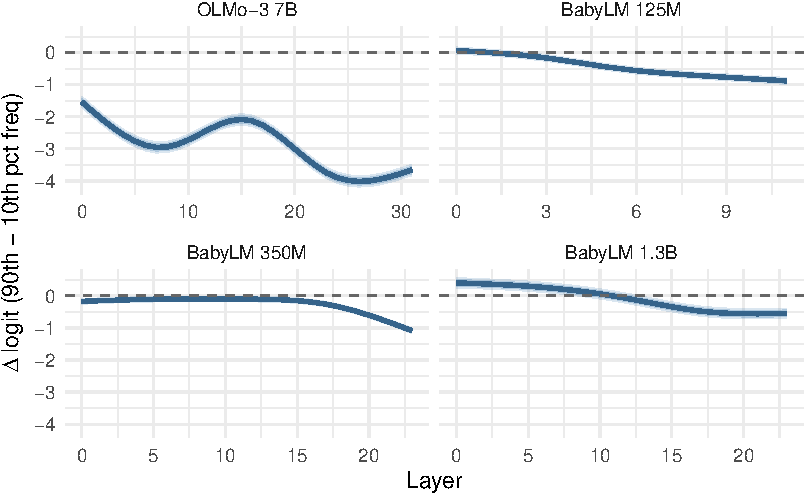
\includegraphics[keepaspectratio]{writeup_files/figure-pdf/fig-exp1-freq-1.pdf}}

}

\caption{\label{fig-exp1-freq}Estimated frequency effect (difference in
predicted logit between the 90th and 10th percentile of log frequency)
across layers for UP independently. Ribbons show 80\% and 95\%
confidence intervals. Panels show OLMo-3 7B and BabyLM models of
increasing size.}

\end{figure}%

\subsection{FTP effect across layers}\label{ftp-effect-across-layers}

\begin{figure}

\centering{

\pandocbounded{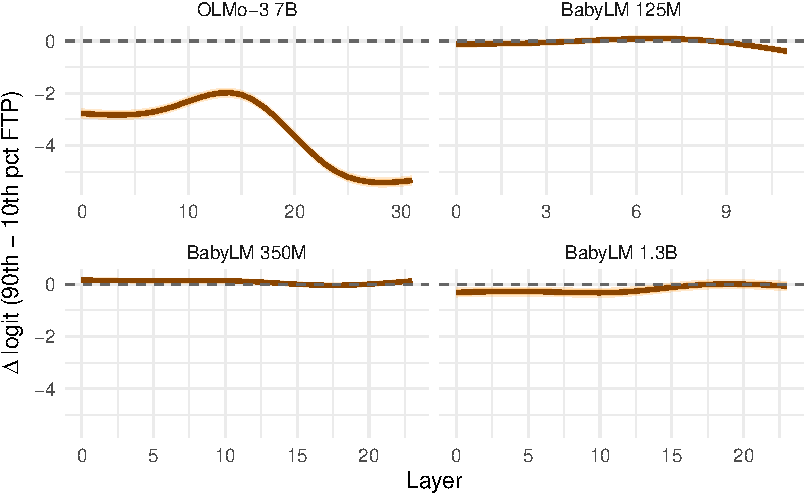
\includegraphics[keepaspectratio]{writeup_files/figure-pdf/fig-exp1-ftp-1.pdf}}

}

\caption{\label{fig-exp1-ftp}Estimated FTP effect (difference in
predicted logit between the 90th and 10th percentile of log-odds FTP)
across layers for UP independently. Ribbons show 80\% and 95\%
confidence intervals. Panels show OLMo-3 7B and BabyLM models of
increasing size.}

\end{figure}%

\section{Experiment 2: UP as Subword}\label{experiment-2-up-as-subword}

\subsection{Items}\label{items-1}

The training set for this experiment combined two types of positive
example: 1,000 occurrences of standalone \emph{up} (identical to
Experiment 1) and 1,000 occurrences of \emph{up} embedded within a
larger word (e.g., \emph{update}, \emph{upon}, \emph{setup}).
Critically, the subword positives were restricted to \textbf{unique word
types}: each up-containing word form contributed exactly one instance,
so the classifier could not learn to recognise a high-frequency form
like \emph{setup} from repeated exposure. Negative examples (1,000 drawn
from each sentence pool) were tokens consisting entirely of alphabetic
characters that did not contain \emph{up} as a substring. The validation
set was constructed by the same procedure (targeting 1,000 positive,
1,000 negative per sentence pool; exact counts vary by tokenizer --- see
Table~\ref{tbl-exp2-splits}). As in Experiment 1, OLMo-3 7B and BabyLM
models used the same underlying sentences with their own tokenizers, and
BabyLM models used BabyLM-corpus statistics for frequency and FTP. The
test set was identical to Experiment 1: all verb--\emph{up} phrasal verb
types with at least 20 corpus occurrences, sampled at up to 20 sentences
per type.

Split sizes by model are shown in Table~\ref{tbl-exp2-splits}. The OLMo
training set contained 1,000 unique up-within-word types; BabyLM models
similarly contributed 1,000 unique types, with the exact set varying by
tokenizer. Validation-set sizes differ slightly across models because
some sentences could not be resolved to a valid token position under
each model's tokenizer. Item-level statistics for the test set are
identical to Experiment 1 (same underlying V+up types) and are shown in
Table~\ref{tbl-exp2-items}.

\begin{longtable}[]{@{}
  >{\raggedright\arraybackslash}p{(\linewidth - 12\tabcolsep) * \real{0.1165}}
  >{\raggedleft\arraybackslash}p{(\linewidth - 12\tabcolsep) * \real{0.1650}}
  >{\raggedleft\arraybackslash}p{(\linewidth - 12\tabcolsep) * \real{0.2816}}
  >{\raggedleft\arraybackslash}p{(\linewidth - 12\tabcolsep) * \real{0.0971}}
  >{\raggedleft\arraybackslash}p{(\linewidth - 12\tabcolsep) * \real{0.0874}}
  >{\raggedleft\arraybackslash}p{(\linewidth - 12\tabcolsep) * \real{0.1456}}
  >{\raggedleft\arraybackslash}p{(\linewidth - 12\tabcolsep) * \real{0.1068}}@{}}

\caption{\label{tbl-exp2-splits}Train, validation, and test split sizes
for Experiment 2 (UP as subword). Positive examples: 1,000 standalone
\emph{up} + 1,000 unique up-within-word types. Negative examples: 1,000
from each sentence pool (standalone and subword). Val sizes vary by
model due to tokenizer coverage.}

\tabularnewline

\toprule\noalign{}
\begin{minipage}[b]{\linewidth}\raggedright
Model
\end{minipage} & \begin{minipage}[b]{\linewidth}\raggedleft
Train standalone
\end{minipage} & \begin{minipage}[b]{\linewidth}\raggedleft
Train subword (unique types)
\end{minipage} & \begin{minipage}[b]{\linewidth}\raggedleft
Train neg
\end{minipage} & \begin{minipage}[b]{\linewidth}\raggedleft
Val rows
\end{minipage} & \begin{minipage}[b]{\linewidth}\raggedleft
Test sentences
\end{minipage} & \begin{minipage}[b]{\linewidth}\raggedleft
Test types
\end{minipage} \\
\midrule\noalign{}
\endhead
\bottomrule\noalign{}
\endlastfoot
OLMo-3 7B & 1,000 & 1,000 & 2,000 & 3,868 & 81,586 & 4,082 \\
BabyLM 125M & 1,000 & 1,000 & 2,000 & 3,582 & 81,543 & 4,082 \\
BabyLM 350M & 1,000 & 1,000 & 2,000 & 3,582 & 81,543 & 4,082 \\
BabyLM 1.3B & 1,000 & 1,000 & 2,000 & 3,773 & 80,425 & 4,081 \\

\end{longtable}

\begin{longtable}[]{@{}
  >{\raggedright\arraybackslash}p{(\linewidth - 12\tabcolsep) * \real{0.1379}}
  >{\raggedleft\arraybackslash}p{(\linewidth - 12\tabcolsep) * \real{0.0920}}
  >{\raggedleft\arraybackslash}p{(\linewidth - 12\tabcolsep) * \real{0.1379}}
  >{\raggedright\arraybackslash}p{(\linewidth - 12\tabcolsep) * \real{0.1494}}
  >{\raggedleft\arraybackslash}p{(\linewidth - 12\tabcolsep) * \real{0.1264}}
  >{\raggedright\arraybackslash}p{(\linewidth - 12\tabcolsep) * \real{0.1839}}
  >{\raggedleft\arraybackslash}p{(\linewidth - 12\tabcolsep) * \real{0.1724}}@{}}

\caption{\label{tbl-exp2-items}Item-level statistics for unique V+up
types in the Experiment 2 test set (identical items to Experiment 1;
same V+up types, same sentences).}

\tabularnewline

\toprule\noalign{}
\begin{minipage}[b]{\linewidth}\raggedright
Model
\end{minipage} & \begin{minipage}[b]{\linewidth}\raggedleft
N items
\end{minipage} & \begin{minipage}[b]{\linewidth}\raggedleft
Median freq
\end{minipage} & \begin{minipage}[b]{\linewidth}\raggedright
Freq range
\end{minipage} & \begin{minipage}[b]{\linewidth}\raggedleft
Median FTP
\end{minipage} & \begin{minipage}[b]{\linewidth}\raggedright
FTP range
\end{minipage} & \begin{minipage}[b]{\linewidth}\raggedleft
Med logit(FTP)
\end{minipage} \\
\midrule\noalign{}
\endhead
\bottomrule\noalign{}
\endlastfoot
BabyLM 125M & 1039 & 920 & 20 -- 390,086 & 0.0325 & 0.00003 -- 0.880 &
-3.40 \\
OLMo-3 7B & 3927 & 92 & 20 -- 390,086 & 0.0046 & 0.00003 -- 0.980 &
-5.38 \\

\end{longtable}

\subsection{Joint model --- first
layer}\label{joint-model-first-layer-1}

\begin{longtable}[]{@{}
  >{\raggedright\arraybackslash}p{(\linewidth - 12\tabcolsep) * \real{0.1667}}
  >{\raggedright\arraybackslash}p{(\linewidth - 12\tabcolsep) * \real{0.2917}}
  >{\raggedleft\arraybackslash}p{(\linewidth - 12\tabcolsep) * \real{0.1250}}
  >{\raggedleft\arraybackslash}p{(\linewidth - 12\tabcolsep) * \real{0.1389}}
  >{\raggedleft\arraybackslash}p{(\linewidth - 12\tabcolsep) * \real{0.0972}}
  >{\raggedleft\arraybackslash}p{(\linewidth - 12\tabcolsep) * \real{0.0972}}
  >{\raggedleft\arraybackslash}p{(\linewidth - 12\tabcolsep) * \real{0.0833}}@{}}

\caption{\label{tbl-exp2-joint-first}Joint frequency × FTP model at the
first layer for UP as subword. Estimates are from Bayesian linear
mixed-effects models (brms); \% \textgreater{} 0 indicates the
percentage of posterior samples with a positive estimate.}

\tabularnewline

\toprule\noalign{}
\begin{minipage}[b]{\linewidth}\raggedright
Model
\end{minipage} & \begin{minipage}[b]{\linewidth}\raggedright
Parameter
\end{minipage} & \begin{minipage}[b]{\linewidth}\raggedleft
Estimate
\end{minipage} & \begin{minipage}[b]{\linewidth}\raggedleft
Est.Error
\end{minipage} & \begin{minipage}[b]{\linewidth}\raggedleft
Q2.5
\end{minipage} & \begin{minipage}[b]{\linewidth}\raggedleft
Q97.5
\end{minipage} & \begin{minipage}[b]{\linewidth}\raggedleft
\% \textgreater{} 0
\end{minipage} \\
\midrule\noalign{}
\endhead
\bottomrule\noalign{}
\endlastfoot
OLMo-3 7B & Intercept & 9.739 & 0.008 & 9.725 & 9.754 & 100.0 \\
OLMo-3 7B & c\_log\_freq & -0.126 & 0.008 & -0.143 & -0.110 & 0.0 \\
OLMo-3 7B & c\_log\_ftp & 0.039 & 0.008 & 0.024 & 0.053 & 100.0 \\
OLMo-3 7B & c\_log\_freq:c\_log\_ftp & -0.019 & 0.008 & -0.034 & -0.004
& 0.7 \\
BabyLM 125M & Intercept & 11.672 & 0.023 & 11.626 & 11.717 & 100.0 \\
BabyLM 125M & c\_log\_freq & 0.054 & 0.023 & 0.008 & 0.100 & 99.0 \\
BabyLM 125M & c\_log\_ftp & -0.053 & 0.023 & -0.097 & -0.007 & 1.1 \\
BabyLM 125M & c\_log\_freq:c\_log\_ftp & -0.003 & 0.024 & -0.050 & 0.044
& 44.3 \\
BabyLM 350M & Intercept & 14.552 & 0.013 & 14.526 & 14.578 & 100.0 \\
BabyLM 350M & c\_log\_freq & -0.116 & 0.013 & -0.142 & -0.089 & 0.0 \\
BabyLM 350M & c\_log\_ftp & 0.098 & 0.014 & 0.071 & 0.125 & 100.0 \\
BabyLM 350M & c\_log\_freq:c\_log\_ftp & -0.003 & 0.014 & -0.030 & 0.024
& 41.6 \\
BabyLM 1.3B & Intercept & 15.297 & 0.030 & 15.239 & 15.356 & 100.0 \\
BabyLM 1.3B & c\_log\_freq & -0.040 & 0.029 & -0.098 & 0.017 & 8.6 \\
BabyLM 1.3B & c\_log\_ftp & 0.012 & 0.029 & -0.044 & 0.071 & 66.0 \\
BabyLM 1.3B & c\_log\_freq:c\_log\_ftp & 0.020 & 0.031 & -0.042 & 0.080
& 73.6 \\

\end{longtable}

\subsection{Joint model --- final
layer}\label{joint-model-final-layer-1}

\begin{longtable}[]{@{}
  >{\raggedright\arraybackslash}p{(\linewidth - 12\tabcolsep) * \real{0.1667}}
  >{\raggedright\arraybackslash}p{(\linewidth - 12\tabcolsep) * \real{0.2917}}
  >{\raggedleft\arraybackslash}p{(\linewidth - 12\tabcolsep) * \real{0.1250}}
  >{\raggedleft\arraybackslash}p{(\linewidth - 12\tabcolsep) * \real{0.1389}}
  >{\raggedleft\arraybackslash}p{(\linewidth - 12\tabcolsep) * \real{0.0972}}
  >{\raggedleft\arraybackslash}p{(\linewidth - 12\tabcolsep) * \real{0.0972}}
  >{\raggedleft\arraybackslash}p{(\linewidth - 12\tabcolsep) * \real{0.0833}}@{}}

\caption{\label{tbl-exp2-joint-final}Joint frequency × FTP model at the
final layer for UP as subword. Estimates are from Bayesian linear
mixed-effects models (brms); \% \textgreater{} 0 indicates the
percentage of posterior samples with a positive estimate.}

\tabularnewline

\toprule\noalign{}
\begin{minipage}[b]{\linewidth}\raggedright
Model
\end{minipage} & \begin{minipage}[b]{\linewidth}\raggedright
Parameter
\end{minipage} & \begin{minipage}[b]{\linewidth}\raggedleft
Estimate
\end{minipage} & \begin{minipage}[b]{\linewidth}\raggedleft
Est.Error
\end{minipage} & \begin{minipage}[b]{\linewidth}\raggedleft
Q2.5
\end{minipage} & \begin{minipage}[b]{\linewidth}\raggedleft
Q97.5
\end{minipage} & \begin{minipage}[b]{\linewidth}\raggedleft
\% \textgreater{} 0
\end{minipage} \\
\midrule\noalign{}
\endhead
\bottomrule\noalign{}
\endlastfoot
OLMo-3 7B & Intercept & 12.316 & 0.042 & 12.235 & 12.400 & 100.0 \\
OLMo-3 7B & c\_log\_freq & -0.449 & 0.047 & -0.542 & -0.358 & 0.0 \\
OLMo-3 7B & c\_log\_ftp & -0.991 & 0.042 & -1.075 & -0.908 & 0.0 \\
OLMo-3 7B & c\_log\_freq:c\_log\_ftp & -0.062 & 0.043 & -0.147 & 0.022 &
7.3 \\
BabyLM 125M & Intercept & 11.731 & 0.075 & 11.584 & 11.878 & 100.0 \\
BabyLM 125M & c\_log\_freq & -0.476 & 0.076 & -0.624 & -0.321 & 0.0 \\
BabyLM 125M & c\_log\_ftp & 0.162 & 0.079 & 0.008 & 0.318 & 98.0 \\
BabyLM 125M & c\_log\_freq:c\_log\_ftp & -0.028 & 0.079 & -0.184 & 0.126
& 36.5 \\
BabyLM 350M & Intercept & 11.229 & 0.073 & 11.086 & 11.375 & 100.0 \\
BabyLM 350M & c\_log\_freq & -0.419 & 0.073 & -0.565 & -0.277 & 0.0 \\
BabyLM 350M & c\_log\_ftp & 0.159 & 0.073 & 0.015 & 0.304 & 98.4 \\
BabyLM 350M & c\_log\_freq:c\_log\_ftp & 0.063 & 0.079 & -0.089 & 0.220
& 79.4 \\
BabyLM 1.3B & Intercept & 9.908 & 0.062 & 9.789 & 10.031 & 100.0 \\
BabyLM 1.3B & c\_log\_freq & -0.240 & 0.061 & -0.363 & -0.123 & 0.0 \\
BabyLM 1.3B & c\_log\_ftp & -0.234 & 0.061 & -0.356 & -0.116 & 0.0 \\
BabyLM 1.3B & c\_log\_freq:c\_log\_ftp & -0.033 & 0.064 & -0.161 & 0.091
& 30.0 \\

\end{longtable}

\subsection{Joint model --- predicted surfaces
(linear)}\label{joint-model-predicted-surfaces-linear-1}

\begin{figure}

\centering{

\pandocbounded{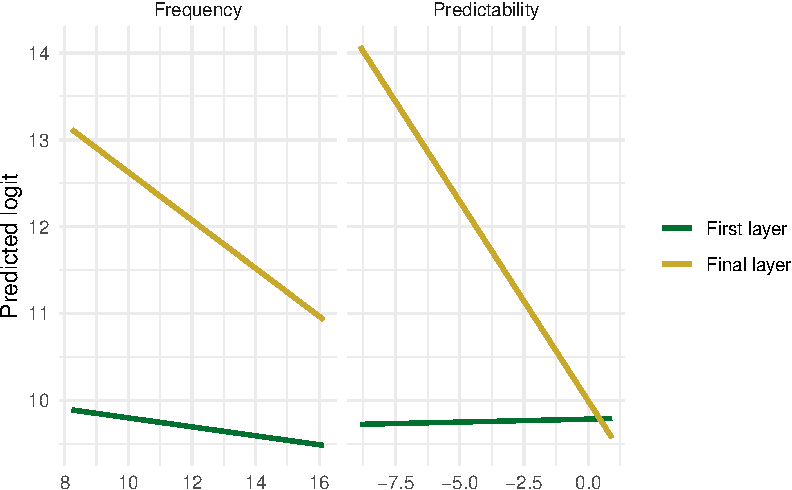
\includegraphics[keepaspectratio]{writeup_files/figure-pdf/fig-exp2-joint-surfaces-1.pdf}}

}

\caption{\label{fig-exp2-joint-surfaces}Predicted logit surfaces from
the linear joint brms model at the first and final layers for OLMo-3 7B
(UP as subword).}

\end{figure}%

\begin{figure}

\centering{

\pandocbounded{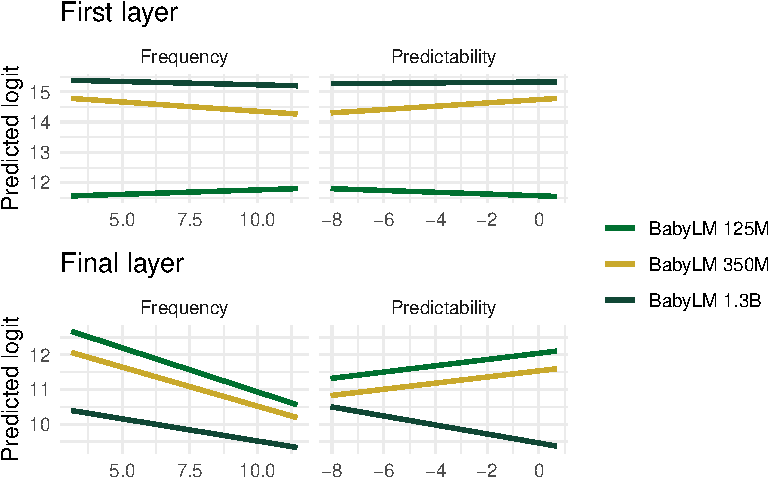
\includegraphics[keepaspectratio]{writeup_files/figure-pdf/fig-exp2-joint-surfaces-blm-1.pdf}}

}

\caption{\label{fig-exp2-joint-surfaces-blm}Predicted logit surfaces
from the linear joint brms model at the first and final layers for
BabyLM models (UP as subword).}

\end{figure}%

\subsection{Polynomial joint model --- first
layer}\label{polynomial-joint-model-first-layer-1}

\begin{longtable}[]{@{}
  >{\raggedright\arraybackslash}p{(\linewidth - 12\tabcolsep) * \real{0.1667}}
  >{\raggedright\arraybackslash}p{(\linewidth - 12\tabcolsep) * \real{0.2917}}
  >{\raggedleft\arraybackslash}p{(\linewidth - 12\tabcolsep) * \real{0.1250}}
  >{\raggedleft\arraybackslash}p{(\linewidth - 12\tabcolsep) * \real{0.1389}}
  >{\raggedleft\arraybackslash}p{(\linewidth - 12\tabcolsep) * \real{0.0972}}
  >{\raggedleft\arraybackslash}p{(\linewidth - 12\tabcolsep) * \real{0.0972}}
  >{\raggedleft\arraybackslash}p{(\linewidth - 12\tabcolsep) * \real{0.0833}}@{}}

\caption{\label{tbl-exp2-poly-joint-first}Polynomial joint model (logit
\textasciitilde{} freq + freq² + FTP + FTP² + freq:FTP) at the first
layer for UP as subword. All predictors are centered and scaled. \%
\textgreater{} 0 = percentage of posterior samples with a positive
estimate.}

\tabularnewline

\toprule\noalign{}
\begin{minipage}[b]{\linewidth}\raggedright
Model
\end{minipage} & \begin{minipage}[b]{\linewidth}\raggedright
Parameter
\end{minipage} & \begin{minipage}[b]{\linewidth}\raggedleft
Estimate
\end{minipage} & \begin{minipage}[b]{\linewidth}\raggedleft
Est.Error
\end{minipage} & \begin{minipage}[b]{\linewidth}\raggedleft
Q2.5
\end{minipage} & \begin{minipage}[b]{\linewidth}\raggedleft
Q97.5
\end{minipage} & \begin{minipage}[b]{\linewidth}\raggedleft
\% \textgreater{} 0
\end{minipage} \\
\midrule\noalign{}
\endhead
\bottomrule\noalign{}
\endlastfoot
OLMo-3 7B & Intercept & 9.801 & 0.010 & 9.781 & 9.820 & 100.0 \\
OLMo-3 7B & c\_log\_freq & -0.084 & 0.010 & -0.103 & -0.065 & 0.0 \\
OLMo-3 7B & Ic\_log\_freqE2 & -0.065 & 0.006 & -0.078 & -0.052 & 0.0 \\
OLMo-3 7B & c\_log\_ftp & 0.055 & 0.009 & 0.038 & 0.072 & 100.0 \\
OLMo-3 7B & Ic\_log\_ftpE2 & -0.023 & 0.006 & -0.035 & -0.011 & 0.0 \\
OLMo-3 7B & c\_log\_freq:c\_log\_ftp & 0.043 & 0.010 & 0.023 & 0.062 &
100.0 \\
BabyLM 125M & Intercept & 11.678 & 0.034 & 11.611 & 11.743 & 100.0 \\
BabyLM 125M & c\_log\_freq & 0.060 & 0.024 & 0.014 & 0.107 & 99.3 \\
BabyLM 125M & Ic\_log\_freqE2 & -0.024 & 0.019 & -0.061 & 0.012 & 9.9 \\
BabyLM 125M & c\_log\_ftp & -0.047 & 0.023 & -0.093 & -0.002 & 2.0 \\
BabyLM 125M & Ic\_log\_ftpE2 & 0.017 & 0.015 & -0.013 & 0.047 & 86.6 \\
BabyLM 125M & c\_log\_freq:c\_log\_ftp & -0.004 & 0.026 & -0.055 & 0.047
& 44.4 \\
BabyLM 350M & Intercept & 14.569 & 0.019 & 14.532 & 14.607 & 100.0 \\
BabyLM 350M & c\_log\_freq & -0.116 & 0.014 & -0.143 & -0.089 & 0.0 \\
BabyLM 350M & Ic\_log\_freqE2 & -0.007 & 0.011 & -0.028 & 0.013 &
24.6 \\
BabyLM 350M & c\_log\_ftp & 0.097 & 0.013 & 0.071 & 0.124 & 100.0 \\
BabyLM 350M & Ic\_log\_ftpE2 & -0.010 & 0.009 & -0.028 & 0.007 & 11.8 \\
BabyLM 350M & c\_log\_freq:c\_log\_ftp & 0.004 & 0.015 & -0.025 & 0.033
& 59.9 \\
BabyLM 1.3B & Intercept & 15.316 & 0.043 & 15.233 & 15.401 & 100.0 \\
BabyLM 1.3B & c\_log\_freq & -0.033 & 0.030 & -0.092 & 0.026 & 14.2 \\
BabyLM 1.3B & Ic\_log\_freqE2 & -0.038 & 0.024 & -0.085 & 0.009 & 5.6 \\
BabyLM 1.3B & c\_log\_ftp & 0.019 & 0.030 & -0.039 & 0.078 & 73.8 \\
BabyLM 1.3B & Ic\_log\_ftpE2 & 0.018 & 0.020 & -0.020 & 0.056 & 82.0 \\
BabyLM 1.3B & c\_log\_freq:c\_log\_ftp & 0.022 & 0.033 & -0.044 & 0.086
& 74.4 \\

\end{longtable}

\subsection{Polynomial joint model --- final
layer}\label{polynomial-joint-model-final-layer-1}

\begin{longtable}[]{@{}
  >{\raggedright\arraybackslash}p{(\linewidth - 12\tabcolsep) * \real{0.1667}}
  >{\raggedright\arraybackslash}p{(\linewidth - 12\tabcolsep) * \real{0.2917}}
  >{\raggedleft\arraybackslash}p{(\linewidth - 12\tabcolsep) * \real{0.1250}}
  >{\raggedleft\arraybackslash}p{(\linewidth - 12\tabcolsep) * \real{0.1389}}
  >{\raggedleft\arraybackslash}p{(\linewidth - 12\tabcolsep) * \real{0.0972}}
  >{\raggedleft\arraybackslash}p{(\linewidth - 12\tabcolsep) * \real{0.0972}}
  >{\raggedleft\arraybackslash}p{(\linewidth - 12\tabcolsep) * \real{0.0833}}@{}}

\caption{\label{tbl-exp2-poly-joint-final}Polynomial joint model (logit
\textasciitilde{} freq + freq² + FTP + FTP² + freq:FTP) at the final
layer for UP as subword. All predictors are centered and scaled. \%
\textgreater{} 0 = percentage of posterior samples with a positive
estimate.}

\tabularnewline

\toprule\noalign{}
\begin{minipage}[b]{\linewidth}\raggedright
Model
\end{minipage} & \begin{minipage}[b]{\linewidth}\raggedright
Parameter
\end{minipage} & \begin{minipage}[b]{\linewidth}\raggedleft
Estimate
\end{minipage} & \begin{minipage}[b]{\linewidth}\raggedleft
Est.Error
\end{minipage} & \begin{minipage}[b]{\linewidth}\raggedleft
Q2.5
\end{minipage} & \begin{minipage}[b]{\linewidth}\raggedleft
Q97.5
\end{minipage} & \begin{minipage}[b]{\linewidth}\raggedleft
\% \textgreater{} 0
\end{minipage} \\
\midrule\noalign{}
\endhead
\bottomrule\noalign{}
\endlastfoot
OLMo-3 7B & Intercept & 12.291 & 0.056 & 12.183 & 12.402 & 100.0 \\
OLMo-3 7B & c\_log\_freq & -0.526 & 0.057 & -0.636 & -0.416 & 0.0 \\
OLMo-3 7B & Ic\_log\_freqE2 & 0.073 & 0.036 & 0.002 & 0.143 & 97.8 \\
OLMo-3 7B & c\_log\_ftp & -0.969 & 0.048 & -1.063 & -0.872 & 0.0 \\
OLMo-3 7B & Ic\_log\_ftpE2 & -0.035 & 0.034 & -0.101 & 0.032 & 15.3 \\
OLMo-3 7B & c\_log\_freq:c\_log\_ftp & -0.090 & 0.057 & -0.203 & 0.022 &
5.7 \\
BabyLM 125M & Intercept & 11.720 & 0.109 & 11.502 & 11.934 & 100.0 \\
BabyLM 125M & c\_log\_freq & -0.417 & 0.076 & -0.568 & -0.269 & 0.0 \\
BabyLM 125M & Ic\_log\_freqE2 & -0.224 & 0.062 & -0.344 & -0.105 &
0.0 \\
BabyLM 125M & c\_log\_ftp & 0.231 & 0.075 & 0.085 & 0.381 & 99.9 \\
BabyLM 125M & Ic\_log\_ftpE2 & 0.243 & 0.051 & 0.146 & 0.343 & 100.0 \\
BabyLM 125M & c\_log\_freq:c\_log\_ftp & -0.081 & 0.083 & -0.240 & 0.085
& 16.5 \\
BabyLM 350M & Intercept & 11.293 & 0.107 & 11.085 & 11.508 & 100.0 \\
BabyLM 350M & c\_log\_freq & -0.377 & 0.073 & -0.519 & -0.229 & 0.0 \\
BabyLM 350M & Ic\_log\_freqE2 & -0.194 & 0.059 & -0.311 & -0.079 &
0.0 \\
BabyLM 350M & c\_log\_ftp & 0.203 & 0.076 & 0.055 & 0.352 & 99.6 \\
BabyLM 350M & Ic\_log\_ftpE2 & 0.126 & 0.048 & 0.033 & 0.221 & 99.7 \\
BabyLM 350M & c\_log\_freq:c\_log\_ftp & 0.059 & 0.080 & -0.098 & 0.216
& 76.7 \\
BabyLM 1.3B & Intercept & 9.722 & 0.086 & 9.555 & 9.891 & 100.0 \\
BabyLM 1.3B & c\_log\_freq & -0.203 & 0.061 & -0.324 & -0.084 & 0.0 \\
BabyLM 1.3B & Ic\_log\_freqE2 & -0.045 & 0.049 & -0.141 & 0.051 &
17.9 \\
BabyLM 1.3B & c\_log\_ftp & -0.187 & 0.061 & -0.307 & -0.068 & 0.1 \\
BabyLM 1.3B & Ic\_log\_ftpE2 & 0.239 & 0.040 & 0.161 & 0.318 & 100.0 \\
BabyLM 1.3B & c\_log\_freq:c\_log\_ftp & -0.128 & 0.067 & -0.262 & 0.000
& 2.5 \\

\end{longtable}

\subsection{Polynomial joint model --- predicted
surfaces}\label{polynomial-joint-model-predicted-surfaces-1}

\begin{figure}

\centering{

\pandocbounded{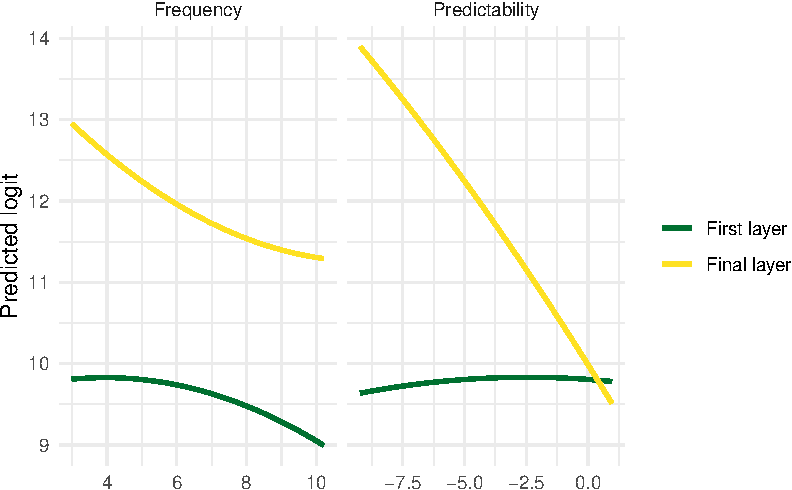
\includegraphics[keepaspectratio]{writeup_files/figure-pdf/fig-exp2-poly-joint-surfaces-1.pdf}}

}

\caption{\label{fig-exp2-poly-joint-surfaces}Predicted logit surfaces
from the polynomial joint brms model at the first and final layers for
OLMo-3 7B (UP as subword).}

\end{figure}%

\begin{figure}

\centering{

\pandocbounded{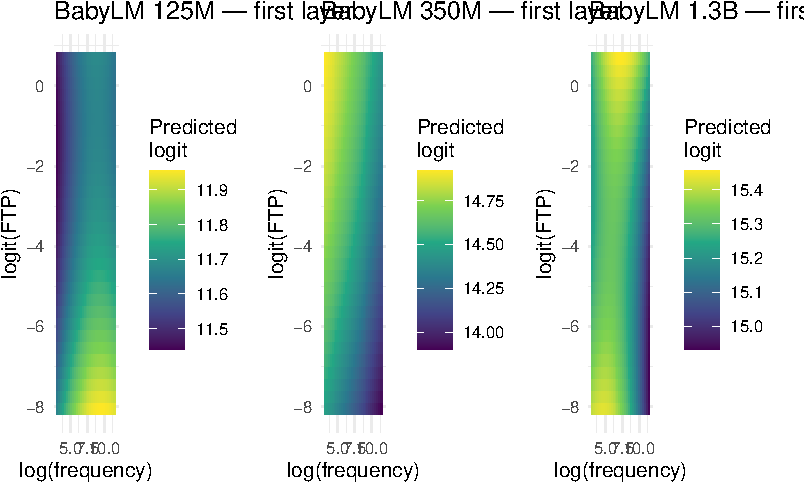
\includegraphics[keepaspectratio]{writeup_files/figure-pdf/fig-exp2-poly-joint-surfaces-blm-1.pdf}}

}

\caption{\label{fig-exp2-poly-joint-surfaces-blm}Predicted logit
surfaces from the polynomial joint brms model at the first and final
layers for BabyLM models (UP as subword).}

\end{figure}%

\subsection{Frequency effect across
layers}\label{frequency-effect-across-layers-1}

\begin{figure}

\centering{

\pandocbounded{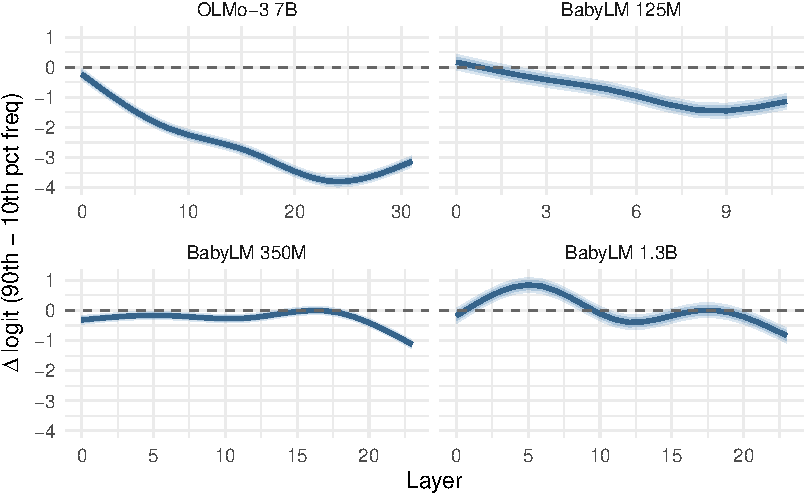
\includegraphics[keepaspectratio]{writeup_files/figure-pdf/fig-exp2-freq-1.pdf}}

}

\caption{\label{fig-exp2-freq}Estimated frequency effect (difference in
predicted logit between the 90th and 10th percentile of log frequency)
across layers for UP as subword. Ribbons show 80\% and 95\% confidence
intervals. Panels show OLMo-3 7B and BabyLM models of increasing size.}

\end{figure}%

\subsection{FTP effect across layers}\label{ftp-effect-across-layers-1}

\begin{figure}

\centering{

\pandocbounded{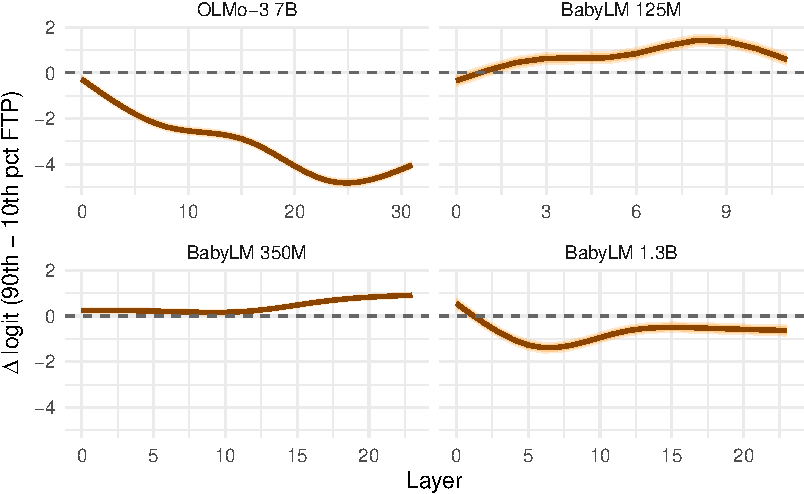
\includegraphics[keepaspectratio]{writeup_files/figure-pdf/fig-exp2-ftp-1.pdf}}

}

\caption{\label{fig-exp2-ftp}Estimated FTP effect (difference in
predicted logit between the 90th and 10th percentile of log-odds FTP)
across layers for UP as subword. Ribbons show 80\% and 95\% confidence
intervals. Panels show OLMo-3 7B and BabyLM models of increasing size.}

\end{figure}%

\section{Experiment 3: Whisper (ASR
Model)}\label{experiment-3-whisper-asr-model}

\subsection{Items}\label{items-2}

The Whisper experiment used spoken language data drawn from a
mixed-source audio metadata file (\texttt{up-audio-metadata.csv})
containing 224,118 timestamped speech segments in which \emph{up}
occurred. Word-level timestamps within each segment were obtained using
WhisperX forced alignment. Each occurrence of \emph{up} was classified
by running spaCy part-of-speech tagging on the full segment transcript:
if the token immediately preceding \emph{up} was tagged as a VERB, the
instance was labelled \emph{V+up} (e.g., \emph{pick up}, \emph{clean
up}); otherwise it was labelled \emph{word\_up} (e.g., \emph{it up},
\emph{them up}). This classification procedure mirrors the one used to
identify standalone \emph{up} in Experiments 1 and 2. Of the 224,118
segments, 58,751 were classified as \emph{word\_up} and 165,367 as
\emph{V+up}, spanning 4,161 unique V+up types.

The \textbf{training and validation sets} used 1,000 \emph{word\_up}
instances each as positive examples, paired with 1,000 randomly selected
non-\emph{up} words from the same segment as negative examples. This
mirrors the standalone-\emph{up} training design of Experiments 1 and 2.
Negative words were restricted to those whose string consists entirely
of alphabetic characters (matching the \texttt{token.isalpha()}
criterion used in Experiments 1 and 2), with a minimum duration of 20
ms. Training and validation segments were non-overlapping.

The \textbf{test set} comprised V+up phrasal verb types with at least 5
occurrences in the audio dataset, yielding 1,466 qualifying types, with
up to 20 instances per type (median: 16 sentences per type; range:
5--20). The minimum-occurrence threshold is lower than in Experiments 1
and 2 (which required at least 20 corpus sentences per type), reflecting
the sparser coverage of audio relative to written text. Corpus frequency
and FTP values were drawn from the C4-derived lookup table used in
Experiments 1 and 2. Split sizes are shown in
Table~\ref{tbl-exp3-splits} and item-level statistics for the Whisper
test set are shown in Table~\ref{tbl-exp3-items}.

\begin{longtable}[]{@{}
  >{\raggedright\arraybackslash}p{(\linewidth - 14\tabcolsep) * \real{0.1176}}
  >{\raggedleft\arraybackslash}p{(\linewidth - 14\tabcolsep) * \real{0.1176}}
  >{\raggedleft\arraybackslash}p{(\linewidth - 14\tabcolsep) * \real{0.1176}}
  >{\raggedleft\arraybackslash}p{(\linewidth - 14\tabcolsep) * \real{0.0941}}
  >{\raggedleft\arraybackslash}p{(\linewidth - 14\tabcolsep) * \real{0.0941}}
  >{\raggedleft\arraybackslash}p{(\linewidth - 14\tabcolsep) * \real{0.1765}}
  >{\raggedleft\arraybackslash}p{(\linewidth - 14\tabcolsep) * \real{0.1294}}
  >{\raggedleft\arraybackslash}p{(\linewidth - 14\tabcolsep) * \real{0.1529}}@{}}

\caption{\label{tbl-exp3-splits}Train, validation, and test split sizes
for Experiment 3 (Whisper). Train/val positive examples are
\emph{word\_up} instances; negatives are random non-\emph{up} alphabetic
tokens from the same segment. Encoder and decoder are evaluated on the
same audio segments using the same train/val/test split.}

\tabularnewline

\toprule\noalign{}
\begin{minipage}[b]{\linewidth}\raggedright
Component
\end{minipage} & \begin{minipage}[b]{\linewidth}\raggedleft
Train pos
\end{minipage} & \begin{minipage}[b]{\linewidth}\raggedleft
Train neg
\end{minipage} & \begin{minipage}[b]{\linewidth}\raggedleft
Val pos
\end{minipage} & \begin{minipage}[b]{\linewidth}\raggedleft
Val neg
\end{minipage} & \begin{minipage}[b]{\linewidth}\raggedleft
Test sentences
\end{minipage} & \begin{minipage}[b]{\linewidth}\raggedleft
Test types
\end{minipage} & \begin{minipage}[b]{\linewidth}\raggedleft
Items w/ FTP
\end{minipage} \\
\midrule\noalign{}
\endhead
\bottomrule\noalign{}
\endlastfoot
Encoder & 1,000 & 1,000 & 1,000 & 1,000 & 20,308 & 1,397 & 1,397 \\
Decoder & 1,000 & 1,000 & 1,000 & 1,000 & 20,308 & 1,397 & 1,397 \\

\end{longtable}

\begin{longtable}[]{@{}
  >{\raggedright\arraybackslash}p{(\linewidth - 14\tabcolsep) * \real{0.1000}}
  >{\raggedleft\arraybackslash}p{(\linewidth - 14\tabcolsep) * \real{0.0800}}
  >{\raggedleft\arraybackslash}p{(\linewidth - 14\tabcolsep) * \real{0.1200}}
  >{\raggedright\arraybackslash}p{(\linewidth - 14\tabcolsep) * \real{0.1300}}
  >{\raggedleft\arraybackslash}p{(\linewidth - 14\tabcolsep) * \real{0.1100}}
  >{\raggedright\arraybackslash}p{(\linewidth - 14\tabcolsep) * \real{0.1600}}
  >{\raggedleft\arraybackslash}p{(\linewidth - 14\tabcolsep) * \real{0.1500}}
  >{\raggedleft\arraybackslash}p{(\linewidth - 14\tabcolsep) * \real{0.1500}}@{}}

\caption{\label{tbl-exp3-items}Item-level statistics for unique V+up
types in the Whisper test set by component. Frequency and FTP are from
C4 (identical across components). FTP = P(up \textbar{} V); logit(FTP) =
log(FTP / (1 − FTP)).}

\tabularnewline

\toprule\noalign{}
\begin{minipage}[b]{\linewidth}\raggedright
Component
\end{minipage} & \begin{minipage}[b]{\linewidth}\raggedleft
N items
\end{minipage} & \begin{minipage}[b]{\linewidth}\raggedleft
Median freq
\end{minipage} & \begin{minipage}[b]{\linewidth}\raggedright
Freq range
\end{minipage} & \begin{minipage}[b]{\linewidth}\raggedleft
Median FTP
\end{minipage} & \begin{minipage}[b]{\linewidth}\raggedright
FTP range
\end{minipage} & \begin{minipage}[b]{\linewidth}\raggedleft
Med logit(FTP)
\end{minipage} & \begin{minipage}[b]{\linewidth}\raggedleft
Med sents/type
\end{minipage} \\
\midrule\noalign{}
\endhead
\bottomrule\noalign{}
\endlastfoot
Decoder & 1397 & 683 & 20 -- 390,086 & 0.0172 & 0.00003 -- 0.980 & -4.05
& 16 \\
Encoder & 1397 & 683 & 20 -- 390,086 & 0.0172 & 0.00003 -- 0.980 & -4.05
& 16 \\

\end{longtable}

\subsection{Joint model --- first
layer}\label{joint-model-first-layer-2}

\begin{longtable}[]{@{}
  >{\raggedright\arraybackslash}p{(\linewidth - 12\tabcolsep) * \real{0.1176}}
  >{\raggedright\arraybackslash}p{(\linewidth - 12\tabcolsep) * \real{0.3088}}
  >{\raggedleft\arraybackslash}p{(\linewidth - 12\tabcolsep) * \real{0.1324}}
  >{\raggedleft\arraybackslash}p{(\linewidth - 12\tabcolsep) * \real{0.1471}}
  >{\raggedleft\arraybackslash}p{(\linewidth - 12\tabcolsep) * \real{0.1029}}
  >{\raggedleft\arraybackslash}p{(\linewidth - 12\tabcolsep) * \real{0.1029}}
  >{\raggedleft\arraybackslash}p{(\linewidth - 12\tabcolsep) * \real{0.0882}}@{}}

\caption{\label{tbl-exp3-joint-first}Joint frequency × FTP model at the
first layer for Whisper encoder and decoder. Estimates are from Bayesian
linear mixed-effects models (brms); \% \textgreater{} 0 indicates the
percentage of posterior samples with a positive estimate.}

\tabularnewline

\toprule\noalign{}
\begin{minipage}[b]{\linewidth}\raggedright
Model
\end{minipage} & \begin{minipage}[b]{\linewidth}\raggedright
Parameter
\end{minipage} & \begin{minipage}[b]{\linewidth}\raggedleft
Estimate
\end{minipage} & \begin{minipage}[b]{\linewidth}\raggedleft
Est.Error
\end{minipage} & \begin{minipage}[b]{\linewidth}\raggedleft
Q2.5
\end{minipage} & \begin{minipage}[b]{\linewidth}\raggedleft
Q97.5
\end{minipage} & \begin{minipage}[b]{\linewidth}\raggedleft
\% \textgreater{} 0
\end{minipage} \\
\midrule\noalign{}
\endhead
\bottomrule\noalign{}
\endlastfoot
Encoder & Intercept & 12.448 & 0.062 & 12.326 & 12.569 & 100.0 \\
Encoder & c\_log\_freq & -0.266 & 0.061 & -0.386 & -0.144 & 0.0 \\
Encoder & c\_log\_ftp & 0.311 & 0.064 & 0.186 & 0.435 & 100.0 \\
Encoder & c\_log\_freq:c\_log\_ftp & -0.024 & 0.059 & -0.139 & 0.092 &
33.8 \\
Decoder & Intercept & 9.243 & 0.017 & 9.211 & 9.276 & 100.0 \\
Decoder & c\_log\_freq & 0.043 & 0.016 & 0.011 & 0.075 & 99.4 \\
Decoder & c\_log\_ftp & -0.061 & 0.017 & -0.093 & -0.028 & 0.0 \\
Decoder & c\_log\_freq:c\_log\_ftp & -0.005 & 0.015 & -0.035 & 0.025 &
37.7 \\

\end{longtable}

\subsection{Joint model --- final
layer}\label{joint-model-final-layer-2}

\begin{longtable}[]{@{}
  >{\raggedright\arraybackslash}p{(\linewidth - 12\tabcolsep) * \real{0.1176}}
  >{\raggedright\arraybackslash}p{(\linewidth - 12\tabcolsep) * \real{0.3088}}
  >{\raggedleft\arraybackslash}p{(\linewidth - 12\tabcolsep) * \real{0.1324}}
  >{\raggedleft\arraybackslash}p{(\linewidth - 12\tabcolsep) * \real{0.1471}}
  >{\raggedleft\arraybackslash}p{(\linewidth - 12\tabcolsep) * \real{0.1029}}
  >{\raggedleft\arraybackslash}p{(\linewidth - 12\tabcolsep) * \real{0.1029}}
  >{\raggedleft\arraybackslash}p{(\linewidth - 12\tabcolsep) * \real{0.0882}}@{}}

\caption{\label{tbl-exp3-joint-final}Joint frequency × FTP model at the
final layer for Whisper encoder and decoder. Estimates are from Bayesian
linear mixed-effects models (brms); \% \textgreater{} 0 indicates the
percentage of posterior samples with a positive estimate.}

\tabularnewline

\toprule\noalign{}
\begin{minipage}[b]{\linewidth}\raggedright
Model
\end{minipage} & \begin{minipage}[b]{\linewidth}\raggedright
Parameter
\end{minipage} & \begin{minipage}[b]{\linewidth}\raggedleft
Estimate
\end{minipage} & \begin{minipage}[b]{\linewidth}\raggedleft
Est.Error
\end{minipage} & \begin{minipage}[b]{\linewidth}\raggedleft
Q2.5
\end{minipage} & \begin{minipage}[b]{\linewidth}\raggedleft
Q97.5
\end{minipage} & \begin{minipage}[b]{\linewidth}\raggedleft
\% \textgreater{} 0
\end{minipage} \\
\midrule\noalign{}
\endhead
\bottomrule\noalign{}
\endlastfoot
Encoder & Intercept & 9.195 & 0.030 & 9.136 & 9.254 & 100.0 \\
Encoder & c\_log\_freq & 0.108 & 0.030 & 0.049 & 0.166 & 100.0 \\
Encoder & c\_log\_ftp & -0.068 & 0.031 & -0.128 & -0.008 & 1.3 \\
Encoder & c\_log\_freq:c\_log\_ftp & 0.035 & 0.028 & -0.020 & 0.091 &
89.6 \\
Decoder & Intercept & 8.485 & 0.056 & 8.377 & 8.594 & 100.0 \\
Decoder & c\_log\_freq & -0.132 & 0.054 & -0.238 & -0.028 & 0.7 \\
Decoder & c\_log\_ftp & -0.421 & 0.055 & -0.529 & -0.314 & 0.0 \\
Decoder & c\_log\_freq:c\_log\_ftp & -0.067 & 0.050 & -0.167 & 0.032 &
8.8 \\

\end{longtable}

\subsection{Joint model --- predicted surfaces
(linear)}\label{joint-model-predicted-surfaces-linear-2}

\begin{figure}

\centering{

\pandocbounded{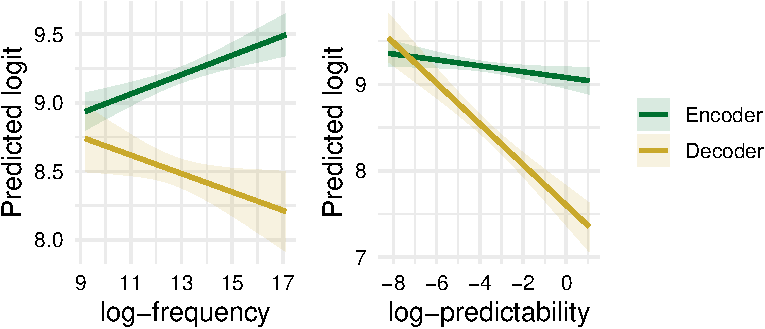
\includegraphics[keepaspectratio]{writeup_files/figure-pdf/fig-exp3-joint-surfaces-1.pdf}}

}

\caption{\label{fig-exp3-joint-surfaces}Predicted logit surfaces from
the linear joint brms model at the first and final layers for Whisper
encoder and decoder.}

\end{figure}%

\subsection{Polynomial joint model --- first
layer}\label{polynomial-joint-model-first-layer-2}

\begin{longtable}[]{@{}
  >{\raggedright\arraybackslash}p{(\linewidth - 12\tabcolsep) * \real{0.1176}}
  >{\raggedright\arraybackslash}p{(\linewidth - 12\tabcolsep) * \real{0.3088}}
  >{\raggedleft\arraybackslash}p{(\linewidth - 12\tabcolsep) * \real{0.1324}}
  >{\raggedleft\arraybackslash}p{(\linewidth - 12\tabcolsep) * \real{0.1471}}
  >{\raggedleft\arraybackslash}p{(\linewidth - 12\tabcolsep) * \real{0.1029}}
  >{\raggedleft\arraybackslash}p{(\linewidth - 12\tabcolsep) * \real{0.1029}}
  >{\raggedleft\arraybackslash}p{(\linewidth - 12\tabcolsep) * \real{0.0882}}@{}}

\caption{\label{tbl-exp3-poly-joint-first}Polynomial joint model (logit
\textasciitilde{} freq + freq² + FTP + FTP² + freq:FTP) at the first
layer for Whisper encoder and decoder. All predictors are centered and
scaled. \% \textgreater{} 0 = percentage of posterior samples with a
positive estimate.}

\tabularnewline

\toprule\noalign{}
\begin{minipage}[b]{\linewidth}\raggedright
Model
\end{minipage} & \begin{minipage}[b]{\linewidth}\raggedright
Parameter
\end{minipage} & \begin{minipage}[b]{\linewidth}\raggedleft
Estimate
\end{minipage} & \begin{minipage}[b]{\linewidth}\raggedleft
Est.Error
\end{minipage} & \begin{minipage}[b]{\linewidth}\raggedleft
Q2.5
\end{minipage} & \begin{minipage}[b]{\linewidth}\raggedleft
Q97.5
\end{minipage} & \begin{minipage}[b]{\linewidth}\raggedleft
\% \textgreater{} 0
\end{minipage} \\
\midrule\noalign{}
\endhead
\bottomrule\noalign{}
\endlastfoot
Encoder & Intercept & 12.478 & 0.083 & 12.313 & 12.641 & 100.0 \\
Encoder & c\_log\_freq & -0.287 & 0.064 & -0.413 & -0.160 & 0.0 \\
Encoder & Ic\_log\_freqE2 & 0.025 & 0.051 & -0.072 & 0.124 & 69.4 \\
Encoder & c\_log\_ftp & 0.339 & 0.068 & 0.205 & 0.473 & 100.0 \\
Encoder & Ic\_log\_ftpE2 & -0.063 & 0.041 & -0.145 & 0.018 & 6.3 \\
Encoder & c\_log\_freq:c\_log\_ftp & 0.001 & 0.077 & -0.150 & 0.153 &
50.4 \\
Decoder & Intercept & 9.291 & 0.022 & 9.248 & 9.335 & 100.0 \\
Decoder & c\_log\_freq & 0.030 & 0.017 & -0.002 & 0.063 & 96.4 \\
Decoder & Ic\_log\_freqE2 & -0.032 & 0.013 & -0.058 & -0.006 & 0.8 \\
Decoder & c\_log\_ftp & -0.039 & 0.018 & -0.074 & -0.002 & 1.8 \\
Decoder & Ic\_log\_ftpE2 & -0.030 & 0.011 & -0.050 & -0.009 & 0.3 \\
Decoder & c\_log\_freq:c\_log\_ftp & 0.039 & 0.021 & -0.001 & 0.080 &
97.1 \\

\end{longtable}

\subsection{Polynomial joint model --- final
layer}\label{polynomial-joint-model-final-layer-2}

\begin{longtable}[]{@{}
  >{\raggedright\arraybackslash}p{(\linewidth - 12\tabcolsep) * \real{0.1176}}
  >{\raggedright\arraybackslash}p{(\linewidth - 12\tabcolsep) * \real{0.3088}}
  >{\raggedleft\arraybackslash}p{(\linewidth - 12\tabcolsep) * \real{0.1324}}
  >{\raggedleft\arraybackslash}p{(\linewidth - 12\tabcolsep) * \real{0.1471}}
  >{\raggedleft\arraybackslash}p{(\linewidth - 12\tabcolsep) * \real{0.1029}}
  >{\raggedleft\arraybackslash}p{(\linewidth - 12\tabcolsep) * \real{0.1029}}
  >{\raggedleft\arraybackslash}p{(\linewidth - 12\tabcolsep) * \real{0.0882}}@{}}

\caption{\label{tbl-exp3-poly-joint-final}Polynomial joint model (logit
\textasciitilde{} freq + freq² + FTP + FTP² + freq:FTP) at the final
layer for Whisper encoder and decoder. All predictors are centered and
scaled. \% \textgreater{} 0 = percentage of posterior samples with a
positive estimate.}

\tabularnewline

\toprule\noalign{}
\begin{minipage}[b]{\linewidth}\raggedright
Model
\end{minipage} & \begin{minipage}[b]{\linewidth}\raggedright
Parameter
\end{minipage} & \begin{minipage}[b]{\linewidth}\raggedleft
Estimate
\end{minipage} & \begin{minipage}[b]{\linewidth}\raggedleft
Est.Error
\end{minipage} & \begin{minipage}[b]{\linewidth}\raggedleft
Q2.5
\end{minipage} & \begin{minipage}[b]{\linewidth}\raggedleft
Q97.5
\end{minipage} & \begin{minipage}[b]{\linewidth}\raggedleft
\% \textgreater{} 0
\end{minipage} \\
\midrule\noalign{}
\endhead
\bottomrule\noalign{}
\endlastfoot
Encoder & Intercept & 9.117 & 0.040 & 9.039 & 9.195 & 100.0 \\
Encoder & c\_log\_freq & 0.133 & 0.030 & 0.074 & 0.193 & 100.0 \\
Encoder & Ic\_log\_freqE2 & 0.025 & 0.024 & -0.022 & 0.072 & 85.1 \\
Encoder & c\_log\_ftp & -0.108 & 0.032 & -0.172 & -0.045 & 0.0 \\
Encoder & Ic\_log\_ftpE2 & 0.074 & 0.019 & 0.035 & 0.111 & 100.0 \\
Encoder & c\_log\_freq:c\_log\_ftp & -0.032 & 0.036 & -0.104 & 0.039 &
18.7 \\
Decoder & Intercept & 8.271 & 0.073 & 8.127 & 8.410 & 100.0 \\
Decoder & c\_log\_freq & -0.060 & 0.054 & -0.164 & 0.047 & 13.2 \\
Decoder & Ic\_log\_freqE2 & 0.061 & 0.044 & -0.025 & 0.148 & 91.7 \\
Decoder & c\_log\_ftp & -0.534 & 0.059 & -0.649 & -0.418 & 0.0 \\
Decoder & Ic\_log\_ftpE2 & 0.207 & 0.035 & 0.139 & 0.276 & 100.0 \\
Decoder & c\_log\_freq:c\_log\_ftp & -0.252 & 0.067 & -0.384 & -0.120 &
0.0 \\

\end{longtable}

\subsection{Polynomial joint model --- predicted
surfaces}\label{polynomial-joint-model-predicted-surfaces-2}

\begin{figure}

\centering{

\pandocbounded{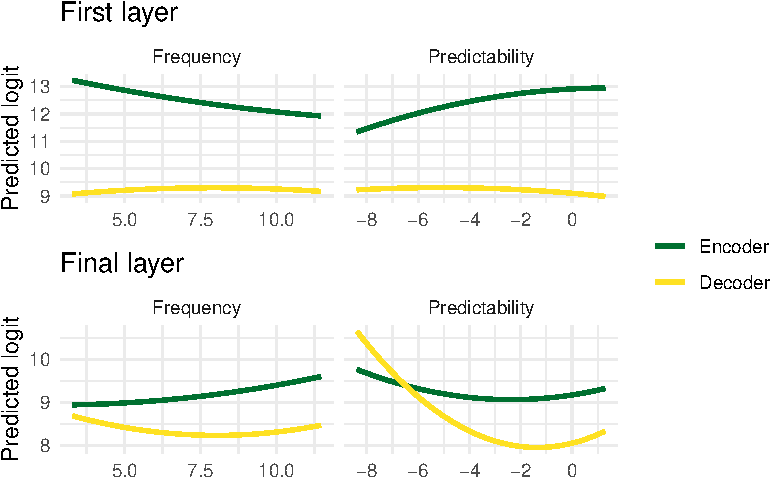
\includegraphics[keepaspectratio]{writeup_files/figure-pdf/fig-exp3-poly-joint-surfaces-1.pdf}}

}

\caption{\label{fig-exp3-poly-joint-surfaces}Predicted logit surfaces
from the polynomial joint brms model at the first and final layers for
Whisper encoder and decoder.}

\end{figure}%

\subsection{Frequency effect across
layers}\label{frequency-effect-across-layers-2}

\begin{figure}

\centering{

\pandocbounded{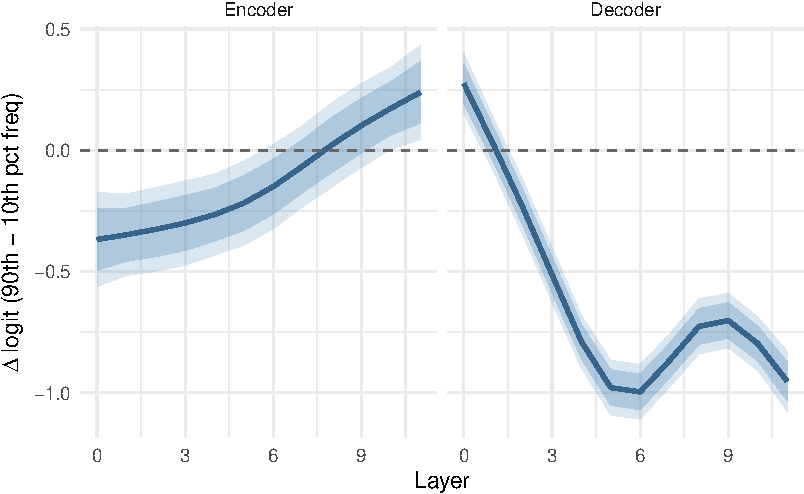
\includegraphics[keepaspectratio]{writeup_files/figure-pdf/fig-exp3-freq-1.pdf}}

}

\caption{\label{fig-exp3-freq}Estimated frequency effect across layers
for Whisper encoder and decoder. Ribbons show 80\% and 95\% confidence
intervals.}

\end{figure}%

\subsection{FTP effect across layers}\label{ftp-effect-across-layers-2}

\begin{figure}

\centering{

\pandocbounded{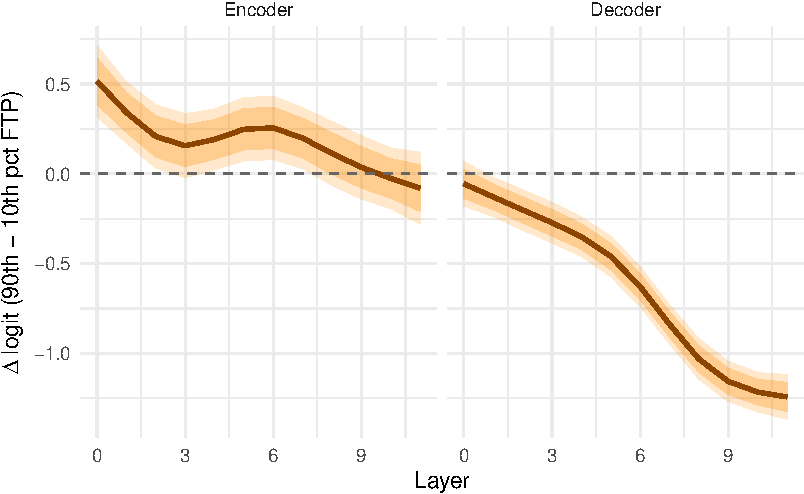
\includegraphics[keepaspectratio]{writeup_files/figure-pdf/fig-exp3-ftp-1.pdf}}

}

\caption{\label{fig-exp3-ftp}Estimated FTP effect across layers for
Whisper encoder and decoder. Ribbons show 80\% and 95\% confidence
intervals.}

\end{figure}%

% acl.sty sets \bibliographystyle{acl_natbib} at load time.
% Only \bibliography{} is needed here to point to the bib file(s).
\bibliography{references.bib}

\end{document}
